\documentclass[autodetect-engine, dvipdfmx-if-dvi, ja=standard]{bxjsarticle}

\usepackage{setspace}        % 行間設定に必要
\usepackage{titlesec}        % titleformatの設定に必要
\usepackage{multicol}        % 2段組みにする
\usepackage{type1cm}         % fontsizeのエラー回避
\usepackage{graphicx}        % 図を表示するのに必要
\usepackage{color}           % jpgなどを表示するのに必要
\usepackage{here}            % 図の配置位置を強制する
\usepackage{amsmath,amssymb} % 数学記号を出すのに必要

% 余白の設定
\setlength{\textheight}{\paperheight}   % 紙面縦幅を本文領域にする(BOTTOM=-TOP)
\setlength{\topmargin}{-15.4truemm}     % 上の余白を10mm(=1inch-15.4mm)に
\addtolength{\topmargin}{-\headheight}  %
\addtolength{\topmargin}{-\headsep}     % ヘッダの分だけ本文領域を移動させる
\addtolength{\textheight}{-20truemm}    % 下の余白も10mm
\setlength{\textwidth}{\paperwidth}     % 紙面横幅を本文領域にする(RIGHT=-LEFT)
\setlength{\oddsidemargin}{-5.4truemm}  % 奇数ページの左の余白を20mm(=1inch-5.4mm)に
\setlength{\evensidemargin}{-5.4truemm} % 偶数数ページの左の余白を20mm(=1inch-5.4mm)に
\addtolength{\textwidth}{-40truemm}     % 右の余白も20mm

% sectionのマージンを調整
\makeatletter
  \renewcommand{\section}{%
    \@startsection{section}{1}{\z@}%
    {0.1\Cvs}{0.1\Cvs}%
    {\normalfont\large\headfont\raggedright}}

  \renewcommand{\subsection}{%
    \@startsection{subsection}{1}{\z@}%
    {0.1\Cvs}{0.1\Cvs}%
    {\normalfont\large\headfont\raggedright}}
\makeatother

% その他設定
\parindent = 0pt                 % 行頭の字下げをしない
\setstretch{1.0}                 % 行間は1文字分
\pagestyle{empty}                % ページ番号を消す
\setlength\textfloatsep{0pt}     % 図の余白
\setlength\abovecaptionskip{0pt} % 図とキャプションの余白
\setlength\intextsep{0pt}
\titleformat*{\section}{\fontsize{11.041pt}{16.562pt}\selectfont \bf}
\titleformat*{\subsection}{\fontsize{11.041pt}{16.562pt}\selectfont \bf}

\begin{document}
\begin{center}
    \fontsize{14.053pt}{21.079pt}\selectfont
    {\bf A02. MATLAB/SimulinkによるRADAR計測システムの開発}\\

    \fontsize{11.041pt}{16.562pt}\selectfont
    佐藤\ 凌雅\ (秋田研究室)
\end{center}

\begin{multicols}{2}
\fontsize{11.041pt}{16.562pt}\selectfont

\section{緒言}
 自動車の走行時に生じる上下方向の振動を抑制する装置としてアクティブサスペンションが開発され,市販車に装備されるまでにその技術は進歩している.しかし,その多くは車両が段差に侵入した際の最初の衝撃を完全に吸収することが困難である.\\
 本研究では,このアクティブサスペンションの動作判定の前段として,路面の段差検知システムの実現を目的とする.提案するシステムはRADARを用いて路面を常に監視し,車両前方の段差の有無を検出する.また,システム構築にはMATLAB/Simulinkを用いたモデルベース開発を採用し,ソフトウェア設計の効率向上を図る.

\section{本論}
 本研究では,路面状態を計測するセンサとしてRADARを用いる.RADARセンサは,Acconeer社製のXC112/XR112評価キットを使用した.この評価キットから得られるデータは距離別の電波の反射強度である.反射強度のピークの位置が路面までの距離となる.このセンサを  図\ref{fig:RADAR_MountingPosition}に示すように分解組立型電気自動車PIUSの前面に路面とのなす角が45度となるように取り付け,本校敷地内にある段差を走行させデータを取得した.

\begin{figure}[H]
  \centering
  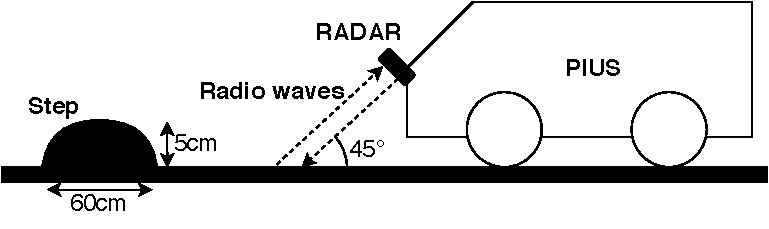
\includegraphics[width=8cm]{./fig/RADAR_MountingPosition.pdf}
  \caption{RADARの取り付け位置}
  \label{fig:RADAR_MountingPosition}
\end{figure}

\subsection{システムの構築}

\begin{figure}[H]
  \centering
  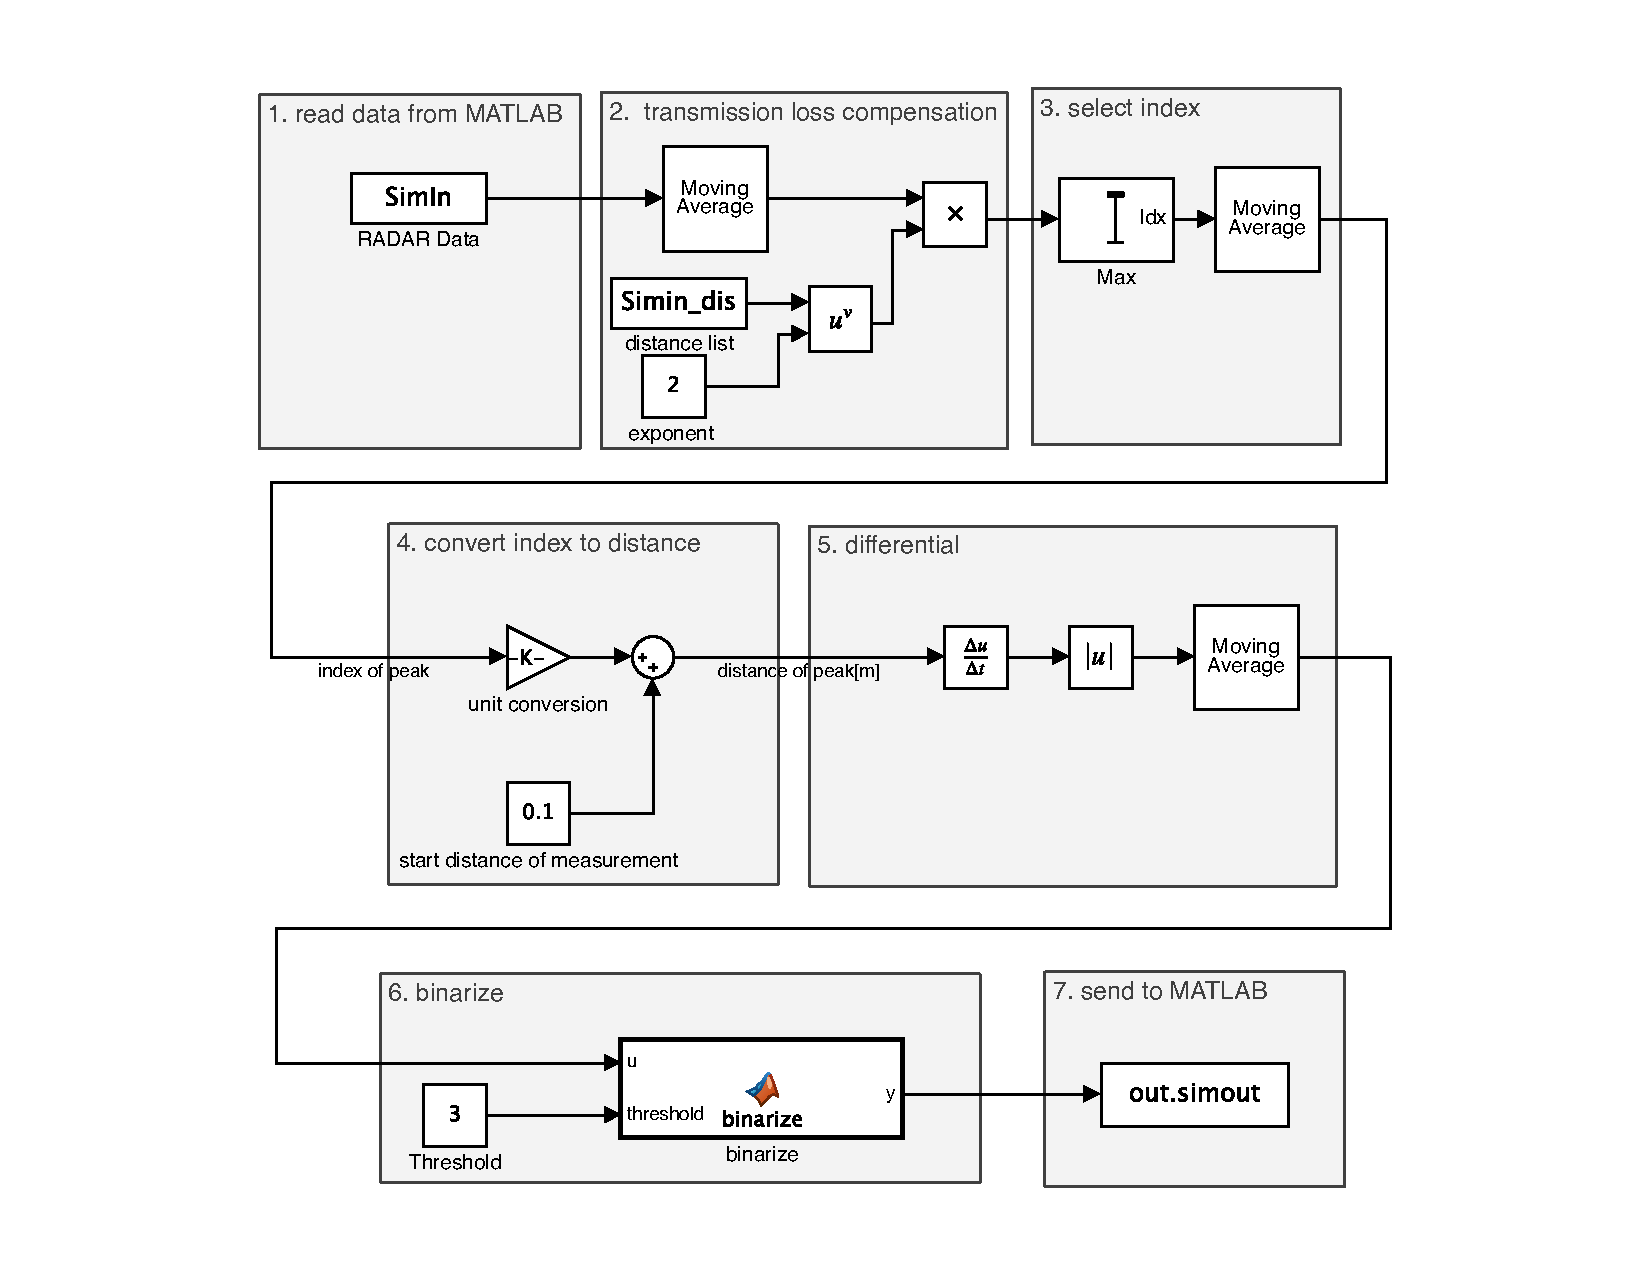
\includegraphics[width=8cm]{./fig/System_Block_BW.pdf}
  \caption{システムブロック図}
  \label{fig:system_block}
\end{figure}

 RADARのデータから路面の段差の有無を検出するためにMATLAB/Simulink上で図\ref{fig:system_block}に示す信号処理アルゴリズムを構築した.アルゴリズムは以下の通りである.\\

\vspace{-8truemm}
\begin{enumerate}
  \item データをMATLABから配列形式で取得
  \item 自由空間での電波の減衰を補償
  \item ピークのインデックスを選択
  \item インデックス番号を実際の距離の単位に変換
  \item 得られた路面までの距離を微分
  \item 微分値を基準に段差検知を判定
\end{enumerate}
\vspace{-2truemm}

\subsection{システムの検証}
 図\ref{fig:result_RADAR}に得られた路面までの距離の微分値を実線で示す.段差判別の閾値は0.7としている.今回は0.405秒と0.610秒の時に段差を検知している.
\begin{figure}[H]
  \centering
  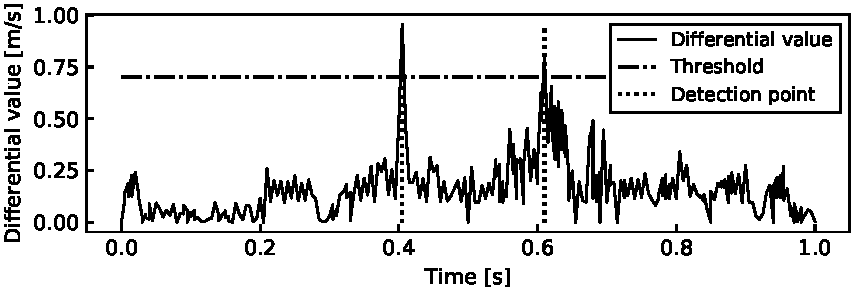
\includegraphics[width=8cm]{./fig/result_RADAR.pdf}
  \caption{測定結果}
  \label{fig:result_RADAR}
\end{figure}
\vspace{-2truemm}

 また,図\ref{fig:result_acc}に測定走行中に車体に加わった上下方向の加速度を実線,システムが段差を検知したタイミングを破線で示す.システムは15m/s$^2$以上の加速度が加わる場合,約50ms前に段差を検知していることがわかる.\\
 しかし,発車時や継続的な振動が加わる場合にも段差が存在すると誤検知していた.これは車両の振動によってセンサの測定値が大きく変動し,それに伴い微分値も増加してしまったためと考えられる.
\begin{figure}[H]
  \centering
  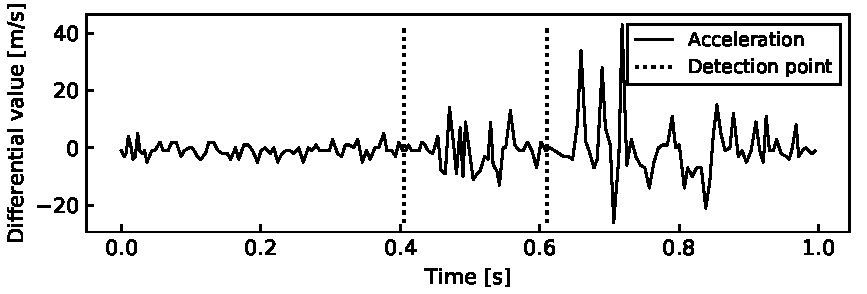
\includegraphics[width=8cm]{./fig/result_acc.pdf}
  \caption{測定結果}
  \label{fig:result_acc}
\end{figure}

\section{結言}
 本研究ではRADARを用いた路面の段差検知のシステムを構築し,検討を行った.RADARを使用することで事前に段差を検知することが可能であることがわかった.また,MATLAB/Simulinkを用いることでシステム構築の速度を向上させることもできた.今後の課題として検知精度の向上や段差の大きさの特定などが挙げられる.
\end{multicols}
\end{document}
